\chapter{Основи мережі Internet}
\nopagebreak[4]
\section*{Мета роботи}
Вивчити основи роботи мережі Інтернет. Ознайомитись з роботою протоколу НТТР. Навчитися встановлювати необхідне програмне забезпечення для розробки сценаріїв на РНР.
\nopagebreak[4]
\section{Структура мережі Internet}
\nopagebreak[4]

\textbf{Інтернет}\index{Мережі!Internet}~--- всесвітня інформаційна комп'ютерна мережа, що являє собою об'єднання безлічі регіональних комп'ютерних мереж і комп'ютерів, що обмінюються один з одним інформацією по каналах громадських телекомунікацій (виділених телефонних аналогових і цифрових лініях, оптичним каналам зв'язку і радіоканалах, в тому числі супутникових лініях зв'язку). Комп'ютери, підключені до мережі Інтернет, можуть мати будь-які апаратні і програмні платформи, але при цьому вони повинні підтримувати стек протоколів (сімейство протоколів) зв'язку TCP/IP.

Інформація в Інтернет зберігається на серверах. Сервери мають свої адреси і управляються спеціалізованим серверним програмним забезпеченням, яке дозволяє пересилати пошту, файли, проводити конференції, тощо. 

Доступ окремих користувачів до інформаційних ресурсів Інтернету зазвичай здійснюється через провайдера або корпоративну мережу.

\textbf{Провайдер (ISP, Internet Service Provider)}\index{Мережі!Internet!провайдер}~--- постачальник мережевих послуг~--- особа або організація надають послуги з підключення до комп'ютерних мереж. В якості провайдера виступає деяка організація, що має модемний пул для з'єднання з клієнтами та виходу у всесвітню мережу. Користувачі підключаються до мережі через маршрутизатори місцевих постачальників послуг Інтернету, які мають постійне підключення до Інтернет через регіональних провайдерів. Регіональний провайдер, підключається до більшого провайдеру національного масштабу, що має вузли в різних містах країни.

Кожен комп'ютер, підключений до мережі Інтернет, має унікальну адресу. Адреси комп'ютерів бувають двох видів:
\begin{enumerate}
\item IP-адреса (обов'язкова)
\item DNS-имя (Domain Name System, доменне ім'я) 
\end{enumerate}
MAC-адреса не розглядається, оскільки у глобальній мережі вона не використовується для ідентифікації комп'ютерів.

\textbf{IP-адрес (Internet Protocol Address)}\index{Мережі!IP}~--— унікальна мережева адреса вузла в комп'ютерній мережі, побудованій на основі IP-протоколу. 
\textbf{IPv4-адреси} складаються з чотирьох байтів, тобто з 32-розрядного двійкового числа, яке для зручності поділяється на чотири блоки по 8 бітів.
\textbf{IPv6-адреси} відображаються як вісім груп по чотири шістнадцяткові цифри, розділені двокрапкою. Приклади IPv4 та IPv6 адрес:

\begin{verbatim}
IPv4: 192.0.2.235
IPv6: 2001:0db8:11a3:09d7:1f34:8a2e:07a0:765d
\end{verbatim}

IP-адреса складається з двох частин: номера мережі й номера вузла (комп'ютера) в мережі. Якщо окремий комп'ютер (хост-комп'ютер) або мережа є складовою частиною мережі Інтернет, то IP-адреса присвоюється організація ICANN (Інтернет корпорація з присвоєння імен і номерів)


\textbf{Доменне (DNS) ім'я}\index{Мережі!DNS}~--- символьне ім'я, що служить для ідентифікації областей~--- одиниць адміністративної автономії в мережі Інтернет~--- у складі вищестоящої по ієрархії такої області. Доменну адресу побудований на основі ієрархічної класифікації, тобто доменну адресу включає в себе кілька рівнів доменів, наприклад: \verb'google.com.ua'.
Домен верхнього рівня розташовується в імені правіше, а домен нижнього рівня~--- лівіше. Користувач мережі Інтернет працює не з IP-адресами, а тільки з доменними адресами. Перетворення доменного імені в IP-адресу здійснюють \textbf{DNS-сервера}.


Для повноцінної роботи в мережі передбачений ряд протоколів прикладного рівня. Протокол прикладного рівня~--- протокол верхнього (7-ого) рівня мережевої моделі OSI, забезпечує взаємодію мережі і користувача. Рівень дозволяє додаткам користувача мати доступ до мережевих служб, таким як обробник запитів до баз даних, доступ до файлів, пересилання електронної пошти. Також відповідає за передачу службової інформації, надає додаткам інформацію про помилки й формує запити до рівня подання. Приклад: HTTP, POP3, SMTP

\pagebreak[3]

\section{Передача даних через протокол HTTP}
\nopagebreak[4]

\textbf{Протокол передачі гіпертексту (Hypertext Transfer Protocol, HTTP)}\index{Мережі!HTTP}~--- протокол прикладного рівня для розподілених мультимедійних інформаційних систем.

Перші версії, такі, як HTTP/0.9, являли собою прості протоколи для передачі даних через Інтернет. Версія HTTP/1.0, поліпшила протокол, дозволивши використання повідомлень в форматі MIME, що містять метаінформацію про переданих даних, і модифікатори для запитів / відгуків.

Для опису характеру, найменування та місця розташування інформаційних ресурсів введені:
\index{Мережі!HTTP!URL/URI/URN} \textbf{URI~--- Uniform Resource Indicator} (уніфікований ідентифікатор ресурсу),
\textbf{URL~--- Uniform Resource Locator} (уніфікований визначник місцезнаходження ресурсу)
\textbf{URN~--- Unifrorm Resource Name} (уніфіковане ім'я ресурсу).
URI: Позначає ім'я та адресу ресурсу в мережі. Як правило ділиться на URL і URN, тому URL і URN це складові URI.

URL: Адреса деякого ресурсу в web. URL визначає місцезнаходження ресурсу і спосіб звертання до нього.

URN: Ім'я деякого ресурсу в web. Сенс URN в тому, що він визначає тільки назва конкретного предмета, який може знаходиться в безлічі конкретних місць.

Як приклад можна представити наступні посилання:
\begin{verbatim}
URI = http://handynotes.ru/2009/09/uri-url-urn.html
URL = http://handynotes.ru
URN = / 2009/09/uri-url-urn.html
\end{verbatim}
HTTP використовується також в якості базового протоколу для комунікації користувацьких агентів з проксі-серверами і іншими системами Інтернет, у тому числі й використовуючих протоколи SMTP, NNTP і FTP.

Всі HTTP-транзакції мають один загальний формат. Кожен запит клієнта і відповідь сервера складається з трьох частин: рядки запиту (відповіді), розділу заголовка і тіла. Клієнт ініціює транзакцію наступним чином:

\begin{enumerate}

\item Клієнт встановлює зв'язок з сервером на номер телефону порту (за замовчуванням~--- 80). Потім клієнт посилає запит документа, вказавши HTTP-команду, яка називається методом, адреса документа і номер версії HTTP. Наприклад, в запиті
\begin{verbatim}
GET / index.html HTTP/1.0
\end{verbatim}

\item Клієнт посилає інформацію заголовка (необов'язкову), щоб повідомити серверу інформацію про свою конфігурації і дані про формати документів, які він може приймати.
\begin{verbatim}
User-Agent: Mozilla/4.05 (WinNT; 1)
Accept: image/gif, image/x-xbitmap, image/jpeg, image/pjpeg, */*
\end{verbatim}

\item Надіславши запит і заголовки, клієнт може відправити і додаткові дані. Клієнти також можуть використовувати їх для приміщення відредагованій сторінки назад на Web-сервер.

\end{enumerate}

Сервер відповідає на запит клієнта наступним чином:

\begin{enumerate}

\item Перша частина відповіді сервера~--- рядок стану, що містить три поля: версію HTTP, код стану й опис. Поле версії містить номер версії HTTP, яку даний сервер користується для передачі відповіді.

Код стану~--- це триразрядне число, що позначає результат обробки сервером запиту клієнта. Опис, наступне за кодом стану, є просто зрозумілий для людини текст, що пояснює код стану. Наприклад, рядок стану \verb'НТТР/1.0 200 OK' говорить про те, що сервер для відповіді використовує версію HTTP 1.0. Код стану 200 означає, що запит клієнта був успішним і витребувані дані будуть передані після заголовків.
\item Після рядка стану сервер передає клієнтові інформацію заголовка, що містить дані про самого сервері і викликаній документі. Нижче наведено приклад заголовка:

\begin{verbatim}
Date: Fri, 10 Jan 1998 08:17:58 GMT
Server: Apache/1.2.6
Last-modified: Mon, 12 Jun 1997 21:53:08 GMT
Content-type: text/html
Content-length: 2482

\end{verbatim}

\item Якщо запит клієнта успішний, то надсилаються витребувані дані. Це може бути копія файлу або результат виконання CGI-програми. Якщо запит клієнта задовольнити не можна, передаються додаткові дані у вигляді зрозумілого для користувача роз'яснення причин, за якими сервер не зміг виконати даний запит.
\end{enumerate}

\pagebreak[3]

\section{Мови програмування для web, web-сервери, мережеві СКБД}
\nopagebreak[4]

\subsection*{Мови програмування}

Серверні мови web-програмування можуть бути умовно розділені по операційним системам, на яких вони працюють: Windows і *nix. Це розділення в деякій мірі умовно, тому що практично всі популярні мови і фреймворки портовано на усі популярні сімейства ОС. Тим не менш, вони рідко використовуються на нерідних ОС.

Якщо говорити про ОС Windows, то тут панує технологія
\textbf{ASP.NET}, \index{Мови програмування!ASP.NET}розроблена компанією Microsoft. За допомогою ASP.NET можна створювати сайти будь-якого рівня складності~--- від найпростіших, що складаються їх декількох сторінок, до дуже складних, що обробляють мільйони запитів на день.

Самим популярним мовою web-програмування є, безумовно,
\textbf{PHP}. \index{Мови програмування!PHP}Його основними перевагами є: простий синтаксис, висока швидкодія, підтримка більшістю хостингів. Дуже вагомою перевагою є те, що на PHP написано багато популярних CMS.

\textbf{Perl}\index{Мови програмування!Perl}~--- це інтерпретована мова програмування. Завдяки цьому, грамотно написаний Perl-скрипт може працювати як в *nix, так і в Windows, як на процесорах x86, так і на Alpha-або Power PC.

\textbf{JSP (Java Server Pages)}\index{Мови програмування!Java Server Pages}~--- це частина технології J2EE, призначена для створення сайтів за допомогою мови Java. JSP має дуже багато спільного з ASP.NET і вибір між цими двома технологіями найчастіше ґрунтується на суб'єктивних перевагах та досвіду роботи з якоюсь іх технологій.

Останнім часом високу популярність придбав мову
\textbf{Ruby}\index{Мови програмування!Ruby} і, зокрема, фреймворк
\textbf{Ruby On Rails}. З його допомогою можна дуже швидко створити сайт з необхідною функціональністю. Одним з істотних недоліків Ruby, є низька швидкодія.

Мова програмування
\textbf{Python}\index{Мови програмування!Python} сьогодні є одною із самих популярних інтерпретованих мов. Python, що є об'єктно-орієнтованою мовою, відмінно справляється з найрізноманітнішими завданнями, а міжплатформенність для цієї мови реалізована в повному обсязі.


\subsection*{Web-сервери}


На даний момент найбільш поширеним web-сервером, що займає більше 65\% ринку, є
\textbf{Apache}\index{Web-сервери!Apache}~--- безкоштовний web-сервер, найбільш часто використовується в UNIX-подібних операційних системах.

У середовищі Windows, дуже поширений
\textbf{IIS (Internet Information Services)}\index{Web-сервери!IIS} від компанії Microsoft, розповсюджуваний з серверними версіями ОС.

\textbf{Nginx}\index{Web-сервери!Nginx}~--- перспективний web-сервер і поштовий проксі-сервер, розроблений для Unix-подібних операційних системах. Починаючи з версії 0.7.52 з'явилася бінарна збірка під Microsoft Windows.

\textbf{Lighttpd}\index{Web-сервери!Lighthttpd}~--- компактний web-сервер, розроблений для Unix-подібних операційних систем, портований надалі на платформу Windows.
\textbf{Google Web Server (GWS)}\index{Web-сервери!GWS}~--- web-сервер, який використовується Google для організації своєї web-інфраструктури.


\subsection*{Мережеві СКБД}


Реляційна модель баз даних являє собою централізоване сховище таблиць, що забезпечує безпечний одночасний доступ до інформації з боку багатьох користувачів. У рядках таблиць частина полів містить дані, що відносяться безпосередньо до запису, а частина~--- посилання на записи інших таблиць. Таким чином, зв'язки між записами є невід'ємною властивістю реляційної моделі.

Кожен запис таблиці має однакову структуру. Наприклад, у таблиці, яка містить описи автомобілів, у всіх записів буде один і той же набір полів: виробник, модель, рік випуску, пробіг і т.д. Такі таблиці легко зображувати в графічному вигляді.

В реляційній моделі СКБД досягається інформаційна та структурна незалежність. Записи не пов'язані між собою настільки, щоб зміна однієї з них торкнулося інші, а зміни структура СКБД, бази даних не обов'язково призводить до перекомпіляції працюючих з нею додатків.
Для побудови сайтів використовують багатокористувацькі реляційні СКБД з підтримкою SQL. Як правило це \index{СУБД}
\textbf{MS SQL Server}, 
\textbf{MySQL, Oracle}, 
\textbf{Interbase}, 
\textbf{DB2} або 
\textbf{PostgreSQL}. Вибір конкретної СКБД залежить від призначення сайту, планованих обсягів бази даних, навантаження на сервер, оптимальної для програміста ліцензії. Величезний відсоток web-хостингів базується на використанні MySQL і PostgreSQL. Цей вибір обумовлений широкими можливостями, наданими даними продуктами, а також їх вартістю.

\pagebreak[3]

\section{Налаштування web-сервера Apache}
\nopagebreak[4]
Завантажити Apache можна з дзеркал наведених на офіційному сайті \verb'http://www.apache.org/'. При пошуку слід пам'ятати, що Apache так само може називатися HTTPD, на ім'я його демона в UNIX. На дзеркалах зазвичай багато різних файлів, необхідно скачати бінарний файл для Windows *.exe або *.msi. У випадку якщо у вас система *nix-сімейства вам необхідно встановити пакет httpd потрібної версії з вашого репозиторію.
Інсталяція програмного пакету для Windows не змінюється вже багато років (Рис.~\ref{f1-1:image}). 
\begin{figure}
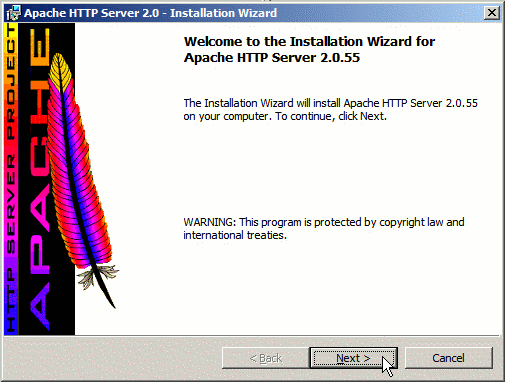
\includegraphics[scale=1,width=8cm]{ch01-01.png}
\caption{Інсталятор Apache}
\label{f1-1:image}
\end{figure}
Вам потрібно буде занести домен, в якому знаходиться сервер, ім'я сервера, e-mail адміністратора сервера. У даному випадку ці дані не важливі, їх можна залишити стандартними  (Рис.~\ref{f1-2:image}).
\begin{figure}
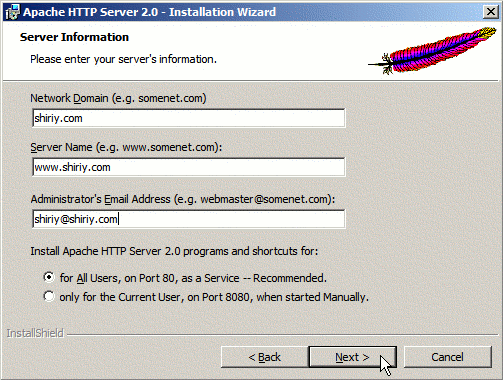
\includegraphics[scale=1,width=8cm]{ch01-02.png}
\caption{Налаштування доменних імен}
\label{f1-2:image}
\end{figure}
Також треба вибрати каталог, куди буде встановлюватися Apache, або залишити його стандартним  (Рис.~\ref{f1-3:image}). 
\begin{figure}
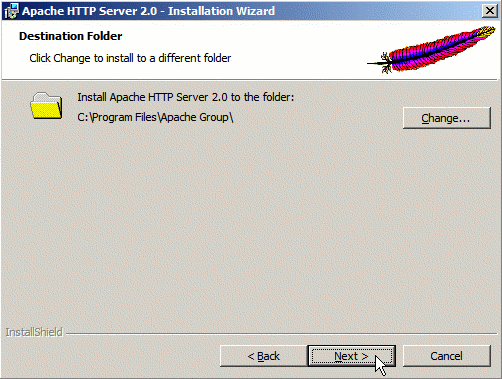
\includegraphics[scale=1,width=8cm]{ch01-03.png}
\caption{Каталог розміщення Apache}
\label{f1-3:image}
\end{figure}
Подальші зміни в конфігурації Apache можна вносити, використовуючи файл <<httpd.conf>>.

Щоб було зручно маніпулювати файлами ваших проектів створіть папку зі зрручним для вас коротким шляхом, наприклад \verb'D:\Site', в якій будуть зберігатися всі інші програми і дані сайту. Далі створіть папку \verb'D:\Site\localhost\', в якій створіть директорії WWW і CGI відповідно. WWW міститиме матеріали сайту, а CGI - скрипти CGI, якщо такі у вас будуть. В директорії \dots\verb'\Apache2\Conf\' знайдіть файл <<httpd.conf>>~--- це файл з налаштуваннями. У ньому знайдіть рядок

\begin{verbatim}
ServerRoot "C :/Program Files/Apache Group/Apache2"
\end{verbatim}

Він повинна містити шлях до самого Апач, тобто на ту папку, куди у вас Апач встановлений. Зверніть увагу, що в шляху слеш прямий і закінчується адреса без слеша.

Далі прив'язуємо Apache до конкретного порту:

\begin{verbatim}
Listen 80
\end{verbatim}

При деяких помилках сервера Apache відсилає електронні листи адміністратору, адреса поштової скриньки налаштовується у рядку

\begin{verbatim}
ServerAdmin your@email.name
\end{verbatim}

Тепер прописуємо шлях до даних сайту

\begin{verbatim}
DocumentRoot "D:/Site/localhost/WWW"
\end{verbatim}

Знайдіть блок 
\begin{verbatim}
<Directory "C:/Program Files/Apache Group/Apache2/htdocs">
\end{verbatim}

і замініть його на

\begin{verbatim}
<Directory "D:/Site">
    Options Indexes Includes
    AllowOverride All
    Order allow,deny
    Allow from all
</Directory>
\end{verbatim}

\pagebreak[3]

\section{Налаштування PHP}
\nopagebreak[4]
Встановлення PHP в середовищі Windows також не створює проблем. Завантажте встановлювач і запустіть його. 

Необхідно буде вибрати каталог для встановлення інтерпретатору, встановлену версію Apache (Рис.~\ref{f1-4:image}).
\begin{figure}
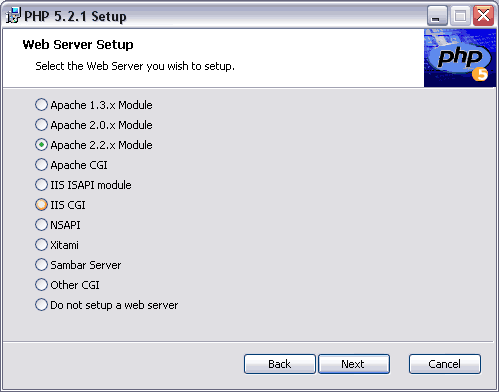
\includegraphics[scale=1,width=8cm]{ch01-04.png}
\caption{Каталог розміщення PHP}
\label{f1-4:image}
\end{figure}
Також необхідно задати місцезнаходження файлу  <<httpd.conf>> (Рис.~\ref{f1-5:image}).
\begin{figure}
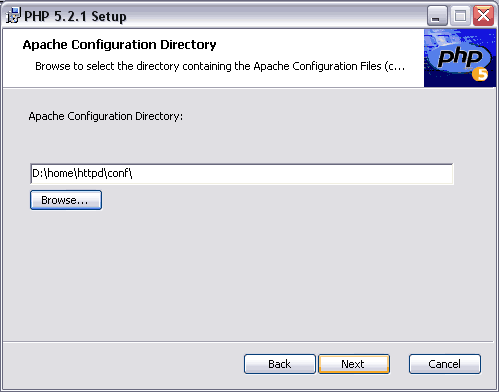
\includegraphics[scale=1,width=8cm]{ch01-05.png}
\caption{Вибір місцезнаходження файлу  <<httpd.conf>>}
\label{f1-5:image}
\end{figure}
Виберіть усі розширення PHP, що йдуть у комплекті, так ви не зіткнетесь з проблемами недостачі бібліотек під час навчання~(Рис.~\ref{f1-6:image}).

\begin{figure}
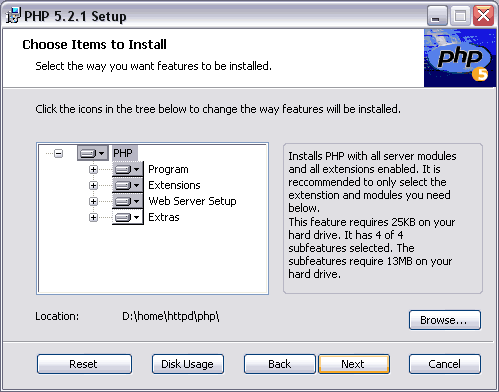
\includegraphics[scale=1,width=8cm]{ch01-06.png}
\caption{Вибір встановлюваних бібліотек}
\label{f1-6:image}
\end{figure}

У випадку проблеми прив'язки PHP до Apache його можна підключити безпосередньо у файлі <<httpd.conf>>. Для цього у файл необхідно додати такі рядки:

\begin{verbatim}
LoadModule php5_module c:/(каталог з PHP)/php5apache2_2.dll 
AddType application/x-httpd-php phtml php
PHPIniDir "c:/(каталог з PHP)/"
\end{verbatim}

Для перевірки роботи PHP та Apache створіть файл у каталозі вашого сайту <<phpinfo.php>> з такими рядками:
\pagebreak[3]
\penalty -20000
\begin{verbatim}
<?php
  echo phpinfo();
?> 
\end{verbatim}

В адресній строці браузера введіть \verb'http://localhost/phpinfo.php'. Якщо ви все виконали правильно, ви повинні побачити сторінку, зображену на Рис.~\ref{f1-7:image}:

\begin{figure}
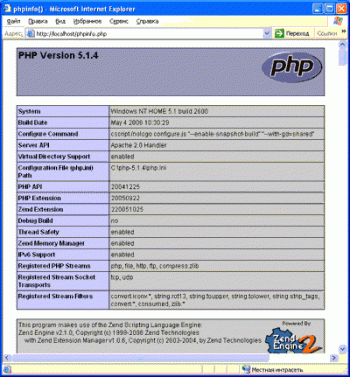
\includegraphics[scale=1,width=8cm]{ch01-07.png}
\caption{Результат роботи функції phpinfo()}
\label{f1-7:image}
\end{figure}

\pagebreak[3]

\section{Налаштування СКБД MySQL}
\nopagebreak[4]
При встановленні  СКБД MySQL вам необхідно запустити файл-інсталятор, даних за замовчуванням достатньо для встановлення повнофункціонального пакету. Після встановлення запуститься майстер налаштувань. Стандартних даних для роботи СКБД достатньо, одначе необхідно буде вказати пароль доступу адміністратора до СКБД в діалозі, зображеному на  Рис.~\ref{f1-8:image}.

\begin{figure}
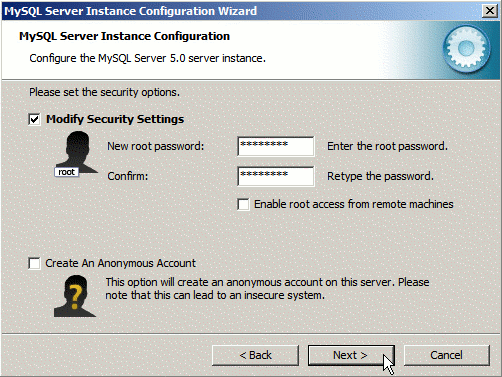
\includegraphics[scale=1,width=8cm]{ch01-08.png}
\caption{Введення пароля адміністратора СКБД}
\label{f1-8:image}
\end{figure}
Після встановлення пароля ви можете під'єднуватися до бази під логіном <<root>> та вказаним вами паролем.

\pagebreak[3]

\section{Індивідуальне завдання}
\nopagebreak[4]
\subsection*{Завдання до лабораторної роботи}
\nopagebreak[4]
\begin{enumerate}
\item Вивчити теоретичний матеріал
\item Відповісти на контрольні запитання
\item Скласти звіт
\item Захистити роботу
\end{enumerate}

\subsection*{Контрольні запитання}
\nopagebreak[4]
\begin{enumerate}
\item Що таке Internet? З яких структурних частин складається Internet?
\item Що таке IP-адреса?
\item Що таке доменне ім'я, з чого воно складається?
\item Який сервіс Internet перетворює IP-адреси в доменні імена і навпаки?
\item Яка служба займається розподіленням блоків IP-адрес?
\item Протокол HTTP. Рівень у моделі OSI, призначення.
\item Значення URI, URL, URN.
\item Мови web-програмування, які ви знаєте.
\item Веб-сервери, які ви знаєте.
\item Мережеві СКБД, які ви знаєте. 
\end{enumerate}



